%\VignetteIndexEntry{choosecolor}
\documentclass{article}\usepackage[]{graphicx}\usepackage[]{color}
%% maxwidth is the original width if it is less than linewidth
%% otherwise use linewidth (to make sure the graphics do not exceed the margin)
\makeatletter
\def\maxwidth{ %
  \ifdim\Gin@nat@width>\linewidth
    \linewidth
  \else
    \Gin@nat@width
  \fi
}
\makeatother

\definecolor{fgcolor}{rgb}{0.345, 0.345, 0.345}
\newcommand{\hlnum}[1]{\textcolor[rgb]{0.686,0.059,0.569}{#1}}%
\newcommand{\hlstr}[1]{\textcolor[rgb]{0.192,0.494,0.8}{#1}}%
\newcommand{\hlcom}[1]{\textcolor[rgb]{0.678,0.584,0.686}{\textit{#1}}}%
\newcommand{\hlopt}[1]{\textcolor[rgb]{0,0,0}{#1}}%
\newcommand{\hlstd}[1]{\textcolor[rgb]{0.345,0.345,0.345}{#1}}%
\newcommand{\hlkwa}[1]{\textcolor[rgb]{0.161,0.373,0.58}{\textbf{#1}}}%
\newcommand{\hlkwb}[1]{\textcolor[rgb]{0.69,0.353,0.396}{#1}}%
\newcommand{\hlkwc}[1]{\textcolor[rgb]{0.333,0.667,0.333}{#1}}%
\newcommand{\hlkwd}[1]{\textcolor[rgb]{0.737,0.353,0.396}{\textbf{#1}}}%

\usepackage{framed}
\makeatletter
\newenvironment{kframe}{%
 \def\at@end@of@kframe{}%
 \ifinner\ifhmode%
  \def\at@end@of@kframe{\end{minipage}}%
  \begin{minipage}{\columnwidth}%
 \fi\fi%
 \def\FrameCommand##1{\hskip\@totalleftmargin \hskip-\fboxsep
 \colorbox{shadecolor}{##1}\hskip-\fboxsep
     % There is no \\@totalrightmargin, so:
     \hskip-\linewidth \hskip-\@totalleftmargin \hskip\columnwidth}%
 \MakeFramed {\advance\hsize-\width
   \@totalleftmargin\z@ \linewidth\hsize
   \@setminipage}}%
 {\par\unskip\endMakeFramed%
 \at@end@of@kframe}
\makeatother

\definecolor{shadecolor}{rgb}{.97, .97, .97}
\definecolor{messagecolor}{rgb}{0, 0, 0}
\definecolor{warningcolor}{rgb}{1, 0, 1}
\definecolor{errorcolor}{rgb}{1, 0, 0}
\newenvironment{knitrout}{}{} % an empty environment to be redefined in TeX

\usepackage{alltt}

\usepackage[round]{natbib} % I want to use bibtex                       



\newtheorem{rexample}{R Example}[section] % I want numbered R examples



\IfFileExists{upquote.sty}{\usepackage{upquote}}{}
\begin{document}
%\SweaveOpts{concordance=TRUE}

\title{aprof: Amdahl's profiler, directed optimization made easy}
\date{\today}
\author{Marco D. Visser}
\maketitle

\abstract{
Amdahl's profiler or \textit{aprof} is meant to assists the evaluation of whether and where to focus code optimization, using Amdahl's law and visual aids based on line profiling. The main goal is to help to balance development vs. execution time. Amdahl's profiler does this by enabling rapid identification of bottnecks within sections of code while simultaniously projecting potential gains. This document explains some of the basic ideas behind aprof: how it applies Amdahl's law to project optimization gains and how it organises profiling output files. It also provides a simple guide towards profiling and code optimization, while identifying somes common inefficiencies in R. 
}


\section{Profiling}
\label{profiling}
\textit{"We should forget about small efficiencies, say about 97\% of the time: premature optimization is the root of all evil"} \\
\newline
- Donald Knuth (1974). "Structured Programming with go to Statements". ACM Journal Computing Surveys 6 (4): 268.
\newline


Empirical studies in computer science show that inefficiency is often rooted in a small proportion of code \citep{Porter1990}.  Therefore, identifying which part of the code takes the most time can allow effective and targeted optimization efforts. “Code profilers” help towards this end; these are software engineering tools that measure the performance of different parts of a program as it executes \citep{Bryant2010}. In this section we will describe how to use a statistical profiler (called $Rprof$ in R), that uses “operating system interrupts” to probe which routines are active at regular intervals and counts which R expressions are consuming the most resources. 

In cases where random-access memory (RAM) storage, rather than processor time, poses the most pressing limit, one can use a memory profiler (e.g. Rprofmem) to obtain similar statistics for memory efficiency. Simpler, though less informative, tools to time and track resource use include the R functions system.time() and object.size(). The former returns the time used by both R and the operating system (for communication between devices, file writing, etc.), while the latter gives an approximation of the memory usage of objects.

Throughout the tutorial we will make heavy use of R's profiling capabilities. R uses a so-called statistical profiler (Rprof), which probes at predefined intervals which routines are active and so we can count which R expressions are consuming most of the system's resources. For example, profiling a program consisting of a two commands will tell you exactly how much time is spent in each command, and therefore which of the two you should take a closer look at. We have also developed software in the form of an R package (aprof: “Amdahl's profiler”) to organize the output from the R profiler using visual tools to identify bottlenecks (as illustrated in Figure \ref{NaiveFigure}). 
  
In this document we will use the package aprof to organise the output from R's standard profiler and makes it much easier to rapidly identify bottlenecks in your program code. An example of using $aprof$ is given below. The package is available at CRAN.

To use this profiler, we first need to make a simple program which we want to profile. Here is an example of a program (InterpreterQuirks) that executes the calculation $N/(1+N)$ many times with either parentheses or brackets, and different amounts of each. The function highlights some of the quirks of an interpreted language as explained earlier (section \ref{whatslowsdown}).

\begin{knitrout}
\definecolor{shadecolor}{rgb}{0.969, 0.969, 0.969}\color{fgcolor}\begin{kframe}
\begin{alltt}
\hlcom{## Rcode7.R}

\hlstd{InterpreterQuirks}\hlkwb{<-}\hlkwa{function}\hlstd{(}\hlkwc{N}\hlstd{)\{}
  \hlkwa{for} \hlstd{(i} \hlkwa{in} \hlnum{1}\hlopt{:}\hlstd{N) \{ N}\hlopt{/}\hlstd{(}\hlnum{1}\hlopt{+}\hlstd{N) \}}
  \hlkwa{for} \hlstd{(i} \hlkwa{in} \hlnum{1}\hlopt{:}\hlstd{N) \{ (((N}\hlopt{/}\hlstd{(}\hlnum{1}\hlopt{+}\hlstd{N))))\}}
  \hlkwa{for} \hlstd{(i} \hlkwa{in} \hlnum{1}\hlopt{:}\hlstd{N) \{ N}\hlopt{/}\hlstd{\{}\hlnum{1}\hlopt{+}\hlstd{N\} \}}
  \hlkwa{for} \hlstd{(i} \hlkwa{in} \hlnum{1}\hlopt{:}\hlstd{N) \{ \{\{\{N}\hlopt{/}\hlstd{\{}\hlnum{1}\hlopt{+}\hlstd{N\}\}\}\} \}}
\hlstd{\}}

\hlcom{## Save the function to a source code file}
\hlkwd{dump}\hlstd{(}\hlstr{"InterpreterQuirks"}\hlstd{,}\hlkwc{file}\hlstd{=}\hlstr{"InterpreterQuirks.R"}\hlstd{)}
\end{alltt}
\end{kframe}
\end{knitrout}

Next we use Rprof to start profiling $InterpreterQuirks$. We will first reload our saved file so the code lines in the R environment, as this ensure that the version in R and the saved file on the disk match up exactly. 

\begin{knitrout}
\definecolor{shadecolor}{rgb}{0.969, 0.969, 0.969}\color{fgcolor}\begin{kframe}
\begin{alltt}
\hlcom{## Rcode8.R}

\hlkwd{source}\hlstd{(}\hlstr{"InterpreterQuirks.R"}\hlstd{)}
\end{alltt}
\end{kframe}
\end{knitrout}

Then we switch on R's profiler $Rprof$, and because we want to know which lines of InterpreterQuirks are the slowest we need to make sure the option $line.profiling$ is set to TRUE. Here we use a time interval between samples of 0.02.

% This should be run outside knitr! Otherwise the profiler
% will include knitr nonsense
\begin{knitrout}
\definecolor{shadecolor}{rgb}{0.969, 0.969, 0.969}\color{fgcolor}\begin{kframe}
\begin{alltt}
\hlcom{## Rcode9.R}

\hlkwd{Rprof}\hlstd{(}\hlkwc{file}\hlstd{=}\hlstr{"InterpreterQuirks.out"}\hlstd{,}\hlkwc{interval} \hlstd{=} \hlnum{0.02}\hlstd{,}
          \hlkwc{line.profiling} \hlstd{=}\hlnum{TRUE}\hlstd{)}

\hlkwd{InterpreterQuirks}\hlstd{(}\hlkwc{N}\hlstd{=}\hlnum{1e5}\hlstd{)} \hlcom{# run 100 thousand times}

\hlkwd{Rprof}\hlstd{(}\hlkwc{append}\hlstd{=F)} \hlcom{# stop profiling}
\end{alltt}
\end{kframe}
\end{knitrout}

Next we load our package $aprof$ ("Amdahl's profiler"). We want to visualize the time spent in each line of code using $aprof$'s standard plot function on our program $InterpreterQuirks$ (see $?plot.aprof$ for details). However before we 
start we need to use the function $aprof$ to make an \textit{"aprof} object". This object will contain the profiling information and the source file $"InterpreterQuirks.R"$. 

\begin{knitrout}
\definecolor{shadecolor}{rgb}{0.969, 0.969, 0.969}\color{fgcolor}\begin{kframe}
\begin{alltt}
\hlcom{## Rcode10.R}

\hlkwd{require}\hlstd{(aprof)}
\end{alltt}


{\ttfamily\noindent\itshape\color{messagecolor}{\#\# Loading required package: aprof}}\begin{alltt}
\hlcom{##make an object of the aprof class}
\hlstd{IntQuirksAprof} \hlkwb{<-} \hlkwd{aprof}\hlstd{(}\hlstr{"InterpreterQuirks.R"}\hlstd{,}\hlstr{"InterpreterQuirks.out"}\hlstd{)}
\end{alltt}


{\ttfamily\noindent\color{warningcolor}{\#\# Warning: cannot open file 'InterpreterQuirks.out': No such file or directory}}

{\ttfamily\noindent\bfseries\color{errorcolor}{\#\# Error: cannot open the connection}}\end{kframe}
\end{knitrout}

Now that we have a standard $"aprof object"$ we can display some basic information about the profiling exercise by simply typing the name of the $"aprof object"$ and hitting return.

\begin{knitrout}
\definecolor{shadecolor}{rgb}{0.969, 0.969, 0.969}\color{fgcolor}\begin{kframe}
\begin{alltt}
\hlcom{## Rcode11.R}

\hlstd{IntQuirksAprof}
\end{alltt}


{\ttfamily\noindent\bfseries\color{errorcolor}{\#\# Error: object 'IntQuirksAprof' not found}}\end{kframe}
\end{knitrout}

Next we can use the standard $plot$ function on this object to display the execution time per line.
The following code should return figure \ref{fig:intquirks}. 

\begin{figure}
\begin{center}
\begin{knitrout}
\definecolor{shadecolor}{rgb}{0.969, 0.969, 0.969}\color{fgcolor}\begin{kframe}
\begin{alltt}
\hlcom{## Rcode12.R}

\hlkwd{plot}\hlstd{(IntQuirksAprof)}
\end{alltt}


{\ttfamily\noindent\bfseries\color{errorcolor}{\#\# Error: object 'IntQuirksAprof' not found}}\end{kframe}
\end{knitrout}
\caption{Output from $aprof$'s PlotExcDens function. It shows the source code for our 
function $InterpreterQuirks$ in the left panel with the execution time per line of code in the right panel. We see a classical interpreted language problem, where more parentheses and brackets mean that the R interpreter has to evaluate more often, while some symbols (here "\{" and "\}") are interpreted faster (i.e. the lookup speed for these symbols is likely faster). Use $profile.plot$ for larger pieces of code. }\label{fig:intquirks}
\end{center}
\end{figure}
\clearpage

Plotting an \textit{aprof} object is useful when your program is relatively small however, when your code consists of hundreds of lines, a better function would be $profile.plot$. Go ahead and use it on our \textit{aprof} object "IntQuirksAprof" to see what it does (type $?profile.plot$ in the command line for details). Another useful feature is to summarize our $aprof$ object, which gives us the theoretical maximum attainable speed-up for each line of code (see $?summary.aprof$ for details). 

\begin{knitrout}\small
\definecolor{shadecolor}{rgb}{0.969, 0.969, 0.969}\color{fgcolor}\begin{kframe}
\begin{alltt}
\hlcom{###Rcode13.R}

\hlkwd{summary}\hlstd{(IntQuirksAprof)}
\end{alltt}


{\ttfamily\noindent\bfseries\color{errorcolor}{\#\# Error: object 'IntQuirksAprof' not found}}\end{kframe}
\end{knitrout}

Using this information we can easily decide where to focus our efforts and, maybe more importantly, decide whether it is worth the effort to optimize the code. As we can see in the uppermost table, line 4 would be the most promising to work on, as it shows the greatest improvement for each of the sets of speed-up factors (1 - 16$\times$). These numbers effectively tell us what the predicted overall speed-up of the program would be when we focus on a single line. That is, if we improve the execution time of a given line by a factor S (S times faster), the table predicts how much this improvement will affect the overall run-time of the entire program. In the above example we see, however, that the gain is minimal and even when the speed-up factor goes to infinity (effectively when the run time of that line becomes 0; $\lim S \to \infty$) we can only achieve a maximum speed-up of 1.39. Or in other words, if we were to infinitely improve the code in line number 4 we would only improve the overall program by 39\%. Infinitely faster is not something we are likely to achieve, but also for the more practical speed-up factors we also see that a factor of 16 improvement is hardly an improvement over a factor of 4. In such cases it may not be worthwhile to either purchase computing resources (parallel machines or execution time on a cluster) or spend time optimizing code. Naturally, in this simple example the overall execution time is so small that we won't spend time optimizing it. However, as we usually would profile a simplified version of a larger program where the execution time may be considerably larger, even a 36\% improvement in execution time may be worthwhile.

\section{Guidelines for optimization}

One should consider optimization only after the code works correctly and produces trustworthy results \citep{Chambers2009}. Once this has been achieved, ask yourself whether cruder code would in the end be more time-efficient? 


It is important to recall a fact that is recognized by programmers:\\
\newline
\textit{"everyone knows that debugging is twice as hard as writing a program in the first place. So if you're as clever as you can be when you write it, how will you ever debug it?"}  \citep{Kernighan1978}.\\ 

Often, only a portion of the code can be optimized. Applying Amdahl’s law \citep{Amdahl1967} can help make the decision of whether to pursue the optimization. Consider a computation that requires time $T_0$ to complete and that we are interested in optimizing a portion of that code. If the portion to optimize requires a fraction $\alpha$ of the total time ($T_0$) to complete, and can be improved by a factor I we can calculate the overall improved execution time ($T_i$) of the entire computation, as:

\begin{equation}
T_i=(1-\alpha) T_0+(\alpha T_0)/I					
\end{equation}

The first term on the right hand side of (1) describes the amount of time required to process the portion of the code that was not optimized. The second term describes the amount of time to process the optimized portion. It follows that the realized speedup factor (S) can be expressed as:

\begin{equation}
S=1 / (( 1 - \alpha )+ \alpha /t)
\end{equation} 		
			
Amdahl's law reveals that the effect of optimization on the overall program performance will depend on both the improvement caused by the optimization (I), and the fraction of the program that can be improved ($\alpha$) (Fig. \ref{fig:amdahl}).  For example, suppose a specific operation within R's program code originally took 50\% of the execution time ($\alpha$ = 0.5), and this operation can be rewritten in a compiled language causing an expected factor 9 speed up (I = 9).  Despite the substantial improvement in the operation, the overall improvement is far less (S = 1.8 times faster). In computer science this is seen as the major insight of Amdahl’s Law \citep{Bryant2010}: unless one improves a very large fraction of the overall system, the realized improvement in execution time will be considerably less. 

\begin{figure}[!ht]
\begin{center}
\begin{knitrout}
\definecolor{shadecolor}{rgb}{0.969, 0.969, 0.969}\color{fgcolor}
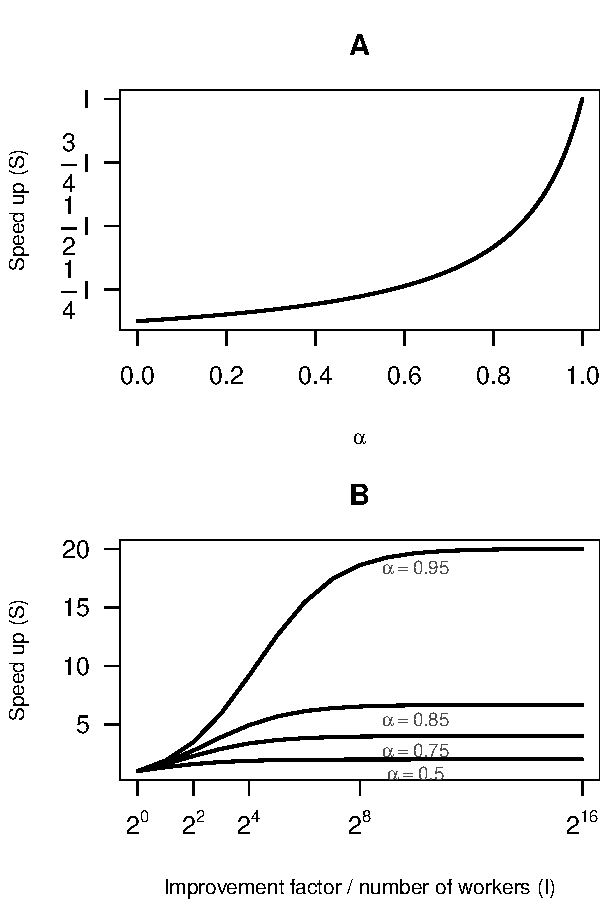
\includegraphics[width=\maxwidth]{figure/Amdahlslaw} 

\end{knitrout}
\caption{
Maximal improvement in program execution speed, or "speed up factor" (S) as predicted by Amdahl's law, either through optimizing code by a factor I or running computations in parallel on I workers. (a) Speed up as function of $\alpha$, the proportion of the total execution time taken up by the section of code, which is improved by factor I. We see that only when a very large fraction ($\alpha$) of the execution time is consumed by the section of code to be optimized, will the overall speed gain come close to I. (b) Total expected speed-up gain for different levels of $\alpha$ as a function of I, which can either represent the improvement factor or number of parallel calculations conducted. We see that there are theoretical limits to the maximal improvement in speed and that it is crucially and asymptotically dependent on $\alpha$. This is also know as the "law of diminishing returns". Predictions based on Amdahl's law are subject to the scaling of the problem. 
} \label{fig:amdahl}
\end{center}
\end{figure} 
 
\clearpage


Here is an example of some basic \textit{aprof} operations, showing the difference in system resources usage between pre-allocating objects in the memory of growing them

\begin{knitrout}
\definecolor{shadecolor}{rgb}{0.969, 0.969, 0.969}\color{fgcolor}\begin{kframe}
\begin{alltt}
\hlkwd{require}\hlstd{(aprof)}
\hlcom{# create function to profile}
     \hlstd{foo} \hlkwb{<-} \hlkwa{function}\hlstd{(}\hlkwc{N}\hlstd{)\{}
             \hlstd{preallocate}\hlkwb{<-}\hlkwd{numeric}\hlstd{(N)}
             \hlstd{grow}\hlkwb{<-}\hlkwa{NULL}
              \hlkwa{for}\hlstd{(i} \hlkwa{in} \hlnum{1}\hlopt{:}\hlstd{N)\{}
                  \hlstd{preallocate[i]}\hlkwb{<-}\hlstd{N}\hlopt{/}\hlstd{(i}\hlopt{+}\hlnum{1}\hlstd{)}
                  \hlstd{grow}\hlkwb{<-}\hlkwd{c}\hlstd{(grow,N}\hlopt{/}\hlstd{(i}\hlopt{+}\hlnum{1}\hlstd{))}
                 \hlstd{\}}
            \hlstd{\}}

     \hlcom{#save function to a source file and reload}
     \hlkwd{dump}\hlstd{(}\hlstr{"foo"}\hlstd{,}\hlkwc{file}\hlstd{=}\hlstr{"foo.R"}\hlstd{)}
     \hlkwd{source}\hlstd{(}\hlstr{"foo.R"}\hlstd{)}


     \hlcom{# Profile the function}
     \hlkwd{Rprof}\hlstd{(}\hlstr{"foo.out"}\hlstd{,}\hlkwc{line.profiling}\hlstd{=}\hlnum{TRUE}\hlstd{)}
     \hlkwd{foo}\hlstd{(}\hlnum{1e2}\hlstd{)}
     \hlkwd{Rprof}\hlstd{(}\hlkwc{append}\hlstd{=}\hlnum{FALSE}\hlstd{)}

     \hlcom{# Create a aprof object}
     \hlstd{fooaprof}\hlkwb{<-}\hlkwd{aprof}\hlstd{(}\hlstr{"foo.R"}\hlstd{,}\hlstr{"foo.out"}\hlstd{)}
\end{alltt}


{\ttfamily\noindent\bfseries\color{errorcolor}{\#\# Error: Rprof outputs appears to be empty, were enough samples made by the profiler?}}\begin{alltt}
     \hlstd{fooaprof}
\end{alltt}


{\ttfamily\noindent\bfseries\color{errorcolor}{\#\# Error: object 'fooaprof' not found}}\end{kframe}
\end{knitrout}

The table above gives some basic output, and shows the lines that were sampled by the profiler, and the amount of time spent in each line. In this simple example it's clear that line 7, takes the most time and should be the target of optimization. This is also shown in the next figure:

\begin{knitrout}
\definecolor{shadecolor}{rgb}{0.969, 0.969, 0.969}\color{fgcolor}\begin{kframe}
\begin{alltt}
\hlkwd{plot}\hlstd{(fooaprof)}
\end{alltt}


{\ttfamily\noindent\bfseries\color{errorcolor}{\#\# Error: object 'fooaprof' not found}}\end{kframe}
\end{knitrout}
\end{document}


